\setchapterimage[6.5cm]{intro_2}
% \setchapterstyle{kao}
\setchapterpreamble[u]{\margintoc}
\chapter[引言]{引言\footnotemark[0]}

\footnotetext{The credits for the image above the chapter title go to:
	Image generated by OpenAI's DALL-E, used in accordance with OpenAI's terms and conditions.}

\section{未来之梦:AI的魔法奇境}

在2025年的某个清晨,随着温暖的阳光透过窗户洒在床上,我从软绵绵的床上醒来,迎接新的一天。我的身体感到前所未有的轻盈,这种感觉很快被我的智能助理的提醒所打断,它温馨地告知我今天的健康监测日程。我在慵懒中伸了一个大大的懒腰,同时智能健康监测设备已经在我醒来的那一刻自动启动,细致地监测我的各项身体指标。这套系统如同一个无形的护卫,日复一日地为我提供全面的健康管理,促使我更加关注并珍视自己的身体健康。

步入厨房,一股清新的香味迎面扑来,我的智能厨具已经开始根据我预设的喜好准备早餐。我通过手腕上的智能手环,轻松选择了一份既美味又健康的早餐菜单,让厨具自动调整食谱以满足我的营养需求。享用早餐不仅是一种味蕾上的享受,更是充满活力开始新一天的关键。这顿精心准备的早餐赋予了我充沛的能量,让我满怀活力地投入到即将展开的每日工作中。

吃早餐时,我的智能财富管家便向我展示了一份详尽的财务管理报告。它深度分析了我的投资组合,考虑到最新的市场趋势和个人风险偏好,提出了精准的优化方案。我仔细审阅了这些建议,并完全认同智能助手的见解,立刻根据这些建议调整了我的投资策略。通过这种科学化的财务管理,我的资产得到了有效的保护和增值,让我对财务的未来充满了信心。结束播报之后,我的智能助理提醒我今天有一场虚拟现实会议,是我与团队的创意讨论。虚拟现实技术的广泛应用已经成为了我们工作中的一部分,使得沟通更加直观、高效。与团队成员们在虚拟现实空间中交流,不仅能够更好地展示各自的创意,还能够更加直观地理解和协作,为项目的进展提供了更多的可能性。

\begin{marginfigure}[-5.5cm]
	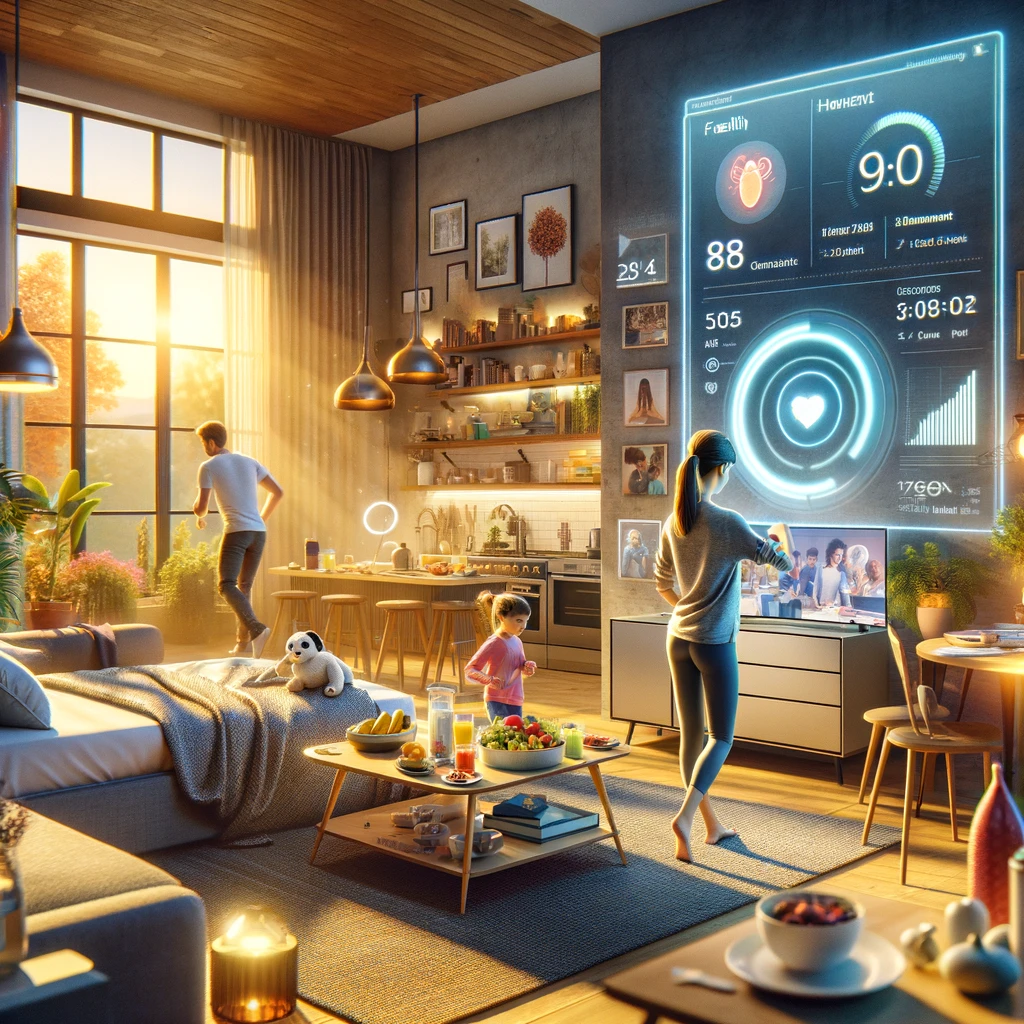
\includegraphics{intro_1.PNG}
	\caption[未来的某个清晨]{未来的某个清晨}
	\label{intro_1}
\end{marginfigure}

早餐后不久,我穿上了智能健身服,这套服装不仅能够监测我的运动数据,还能实时调整锻炼强度,保证我在最佳状态下锻炼。我的智能健身器材根据我的身体状况和健康目标,自动调整了今天的锻炼计划。在运动过程中,智能音乐系统根据我的心率和偏好播放着舒缓的音乐,同时,智能助理还提供心理健康提示,让我的身心同时得到放松和锻炼。

我的孩子们也开始了他们的一天,智能教育系统已经为他们准备好了今日的学习计划。这一系统能够根据他们的学习进度、兴趣爱好推荐适合的学习材料,并通过互动方式让学习变得更加生动有趣。这种个性化的学习方式不仅提高了他们的学习效率,还激发了他们对知识的好奇心。智能家庭教师会实时调整教学内容,确保我的孩子们在最佳的环境中成长。

进入工作状态后,我的智能助理帮我整理了一天的工作日程,并提供了必要的资料和信息。我与我的虚拟团队在虚拟现实空间中开展了会议,利用虚拟现实技术进行头脑风暴和创意讨论。智能家庭教师则帮助我的孩子们在线学习,为他们提供个性化的教育辅导。家庭教育的改变不仅在于学习方式的转变,更在于智能化教育带来的个性化关怀,让每个孩子都能得到最适合他们的教学方式。

工作日的傍晚,我决定去看望父母。我的智能助理不仅即刻规划出了前往父母家的最佳路线,还根据实时交通状况进行了动态调整,确保我能以最快速度到达。我坐进了自动驾驶汽车,它沿着预设路线安静而迅速地穿梭在城市间,将数十公里的距离缩短为仅需的几分钟旅程。

到达父母家时,我通过智能家庭监控系统迅速了解到家中的安全状况及父母的健康情况。这套系统不仅能实时监控家中的安全,还能通过连接的健康监测设备,详细记录并分析父母的健康数据,如心率、血压等重要指标。一旦发现任何异常,系统会立即通知我并提出建议行动,同时智能助手会定期提醒父母按时服药、进行适当的运动,并注意健康饮食,全面保障他们的健康。

回到家中,我被智能家居系统营造的温馨环境所包围。智能灯光根据室内光线自动调整,营造出最舒适的氛围,而智能音乐系统则根据我的心情和偏好播放着轻松愉悦的音乐,让我快速从白天的忙碌中解脱出来,与家人共享宝贵的家庭时光。临睡前,我与我的智能财富管家进行了简短的交流,它根据最新的市场动态为我提供了个性化的理财建议和投资策略,帮助我更好地规划和管理我的财务。

随着智能技术的不断进步,我的生活在各个方面都变得更加智慧和便捷。从健康监测到虚拟现实会议,从个性化学习到创意生产,再到家庭安全和医疗保健,每一项服务都在人工智能的帮助下达到了新的高度。这些技术的融合不仅为我提供了前所未有的便利,也极大地提高了生活的质量和效率。

我深信,在人工智能的引领下,我们将迎来一个更加智慧、美好的未来。这个未来不仅仅是关于技术的进步,更是关于生活方式的革新,让每个人都能享受到更加健康、快乐和安全的生活。随着科技的不断发展,我对未来充满了无限的期待和希望,相信人工智能将继续为我们的生活带来更多的可能性和奇迹。

\section{时光之舞:AI历史交响曲}
\subsection[人工智能概念]{人工智能概念 \sidenote{人工智能是什么、学派有哪些,强人工智能和弱人工智能,人工智能和大脑的关联性}}

人工智能(Artificial Intelligence,简称AI)一词缘于1956年8月美国达特茅斯学院的夏季研讨会。在1955年8月的时候,“人工智能”在一份关于召开国际人工智能会议的提案中被提出,这份提案由东道主约翰·麦卡锡(John McCarthy)、哈佛大学的马文·明斯基(Marvin Minsky)、IBM的纳撒尼尔·罗切斯特(Nathaniel Rochester)、信息论的创始人克劳德·香农(Claude Shannon)联合递交。一年之后,在达特茅斯召开的第一次人工智能大会,而这次会议被认为是开辟了人工智能研究领域的历史性事件,所以一般来说,它的起源要从1956年算起。


人工智能是利用数字计算机或者数字计算机控制的机器模拟、延伸和扩展人的智能,感知环境、获取知识并使用知识获得最佳结果的理论、方法、技术及应用系统。人工智能属于计算机科学的一个分支,研究领域涉及计算机视觉、自然语言处理、搜索与推荐等,同时又与多个学科紧密相关,包括了自动化、电子技术、数学、心理学、语言学、哲学等。

\begin{marginfigure}[-5.5cm]
	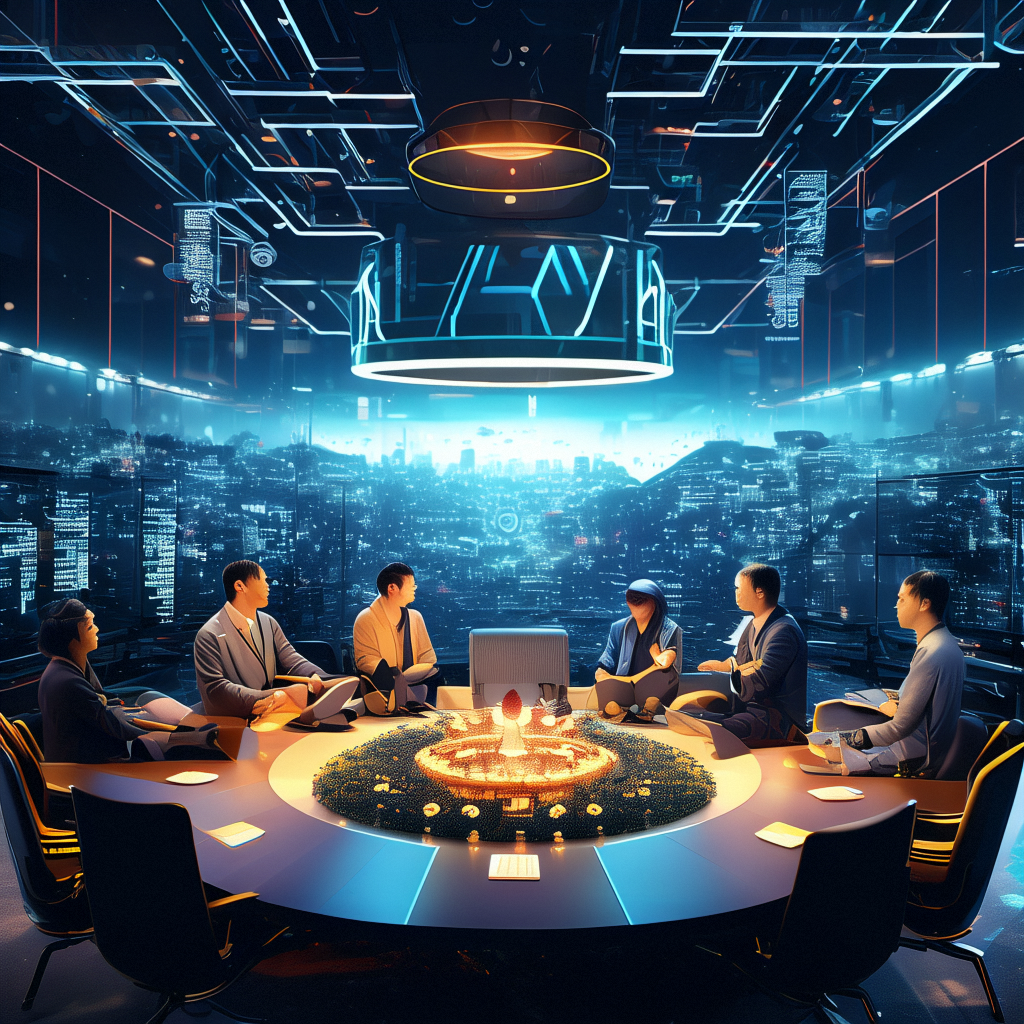
\includegraphics{intro_3.PNG}
\end{marginfigure}

从学术角度来看,人工智能主要包括符号主义、联结主义和行为主义三个学派。其中,符号主义主义的思想起源来自数理逻辑,主张将智能形式化为符号、知识、规则和算法,并用计算机实现符号、知识、规则和算法的表征和计算,从而实现用计算机来模拟人的智能行为,典型的代表算法有决策树;联结主义的思想起源来自衍生学,主张生物智能是由圣经网络产生的,通过人工方式构造神经网络,再训练人工神经网络产生智能,典型的代表算法有神经网络;行为主义的思想起源来自控制论,主张生物智能是自然进化的产物,生物通过与环境及其他生物之间的相互作用,从而发展出越来越强的智能,典型的代表算法有遗传算法和强化学习等。目前,三大学派呈现出逐渐融合的趋势,发挥其各自特点共同持续推动人工智能产业发展。

人工智能可以分为弱人工智能和强人工智能,其中弱人工智能是指不能真正实现推理和解决问题的智能机器,这些机器表面看像是智能的,但是并不真正拥有智能,也不会有自主意识;而强人工智能是指真正能思维的智能机器,并且认为这样的机器是有知觉的和自我意识的,这类机器可分为类人(机器的思考和推理类似人的思维)与非类人(机器产生了和人完全不一样的知觉和意识,使用和人完全不一样的推理方式) 两大类。迄今为止的人工智能系统都还是实现特定功能的专用智能,而不是像人类智能那样能够不断适应复杂的新环境并不断涌现出新的功能,因此都还是弱人工智能。目前的主流研究仍集中于弱人工智能,并取得了显著进步,如语音识别、图像处理和物体分割、机器翻译等方面取得了重大突破,甚至可以接近或超越人类水平。强人工智能不仅在哲学上存在巨大争论(涉及到思维与意识等根本问题的讨论),在技术上的研究也具有极大的挑战性。目前强人工智能鲜有进展,大部分专家任务至少在未来几十年内难以实现。

\subsection[发展历程]{发展历程\sidenote{从国际视角到国内视角,介绍人工智能的主要时间节点}}

人工智能的历史源远流长,许多文明中都有创造人类的神话故事,如西方神话中如赫淮斯托斯的黄金机器人和皮格马利翁的伽拉忒亚,东方神话中的女娲造人等,这些故事反映了是古代人民对于世界和自身存在意义的好奇心和探索欲,是对于存在的深层次思考。现代人工智能的发展不仅是技术进步的体现,更是人类文化和哲学思考的延续。这些古老的神话故事,不仅丰富着我们对人工智能的理解,也指引着我们在技术进步的同时,不忘对人性、生命和存在的反思和尊重。

人工智能的发展从一开始就与计算机科学的发展紧密相连,这种联系可以追溯到计算机科学的早期历史。二战期间,艾伦·图灵的贡献是一个重要的里程碑。图灵不仅帮助英国军方破译了德国军方的著名密码系统Enigma,而且他构造的计算机系统被视为人工智能系统的雏形。图灵的工作展示了计算机不仅可以执行简单的算术运算,还可以进行复杂的逻辑和模式识别任务,这是人工智能的核心能力之一。图灵的贡献还包括他对计算机和人工智能潜力的理论探讨。1948年,他发表的《计算机与智能》论文中提出了著名的“图灵测试”,这是判断机器是否能展现出与人类相似智能的第一个正式标准。图灵测试的提出,不仅推动了人工智能领域的理论研究,也激发了对机器智能可能性的广泛兴趣。图灵的工作不仅为破译代码提供了计算技术,也奠定了现代人工智能研究的基础。他对机器能否思考的探索,以及他开发的技术和理论,都彰显了人工智能作为计算机科学领域内一个长期且核心的研究方向的地方。

人工智能(AI)的历程是一条充满挑战与创新的道路,从理论的萌芽到技术的爆炸式增长,经历了以下六个重要阶段:
\begin{itemize}
    \item 起步发展期(1956年—1960年代初):标志着人工智能概念的正式提出,科学家们在机器定理证明、跳棋程序等领域取得了初步成果,开启了AI研究的首个高潮。
    \item 反思发展期(1960年代—1970年代初):在经历了初期的乐观预期后,更具挑战性的任务揭示了AI技术的局限性,如机器翻译的不足,引发了对AI未来方向的深刻反思。
    \item 应用发展期(1970年代初—1980年代中):专家系统的出现,模拟人类专家解决特定问题的能力,标志着AI从理论走向实际应用的重要突破,尤其在医疗、化学和地质等领域展现了巨大潜力。
    \item 低迷发展期(1980年代中—1990年代中):随着应用的扩大,专家系统的局限性逐渐显现,如知识获取困难、推理方法单一等问题,导致了AI发展的一段低迷期。
    \item 稳步发展期(1990年代中—2010年):网络和互联网技术的飞速发展,特别是IBM深蓝的胜利和“智慧地球”概念的提出,为AI研究注入了新动力,推动技术逐步实用化。
    \item 蓬勃发展期(2011年至今):大数据、云计算等技术的突破,结合深度学习的兴起,极大地推进了AI技术的发展,实现了从理论到实用的巨大跨越,AI技术在图像分类、语音识别等多个领域实现了质的飞跃,迎来了新的高潮。
\end{itemize}

\begin{figure}[htbp]
	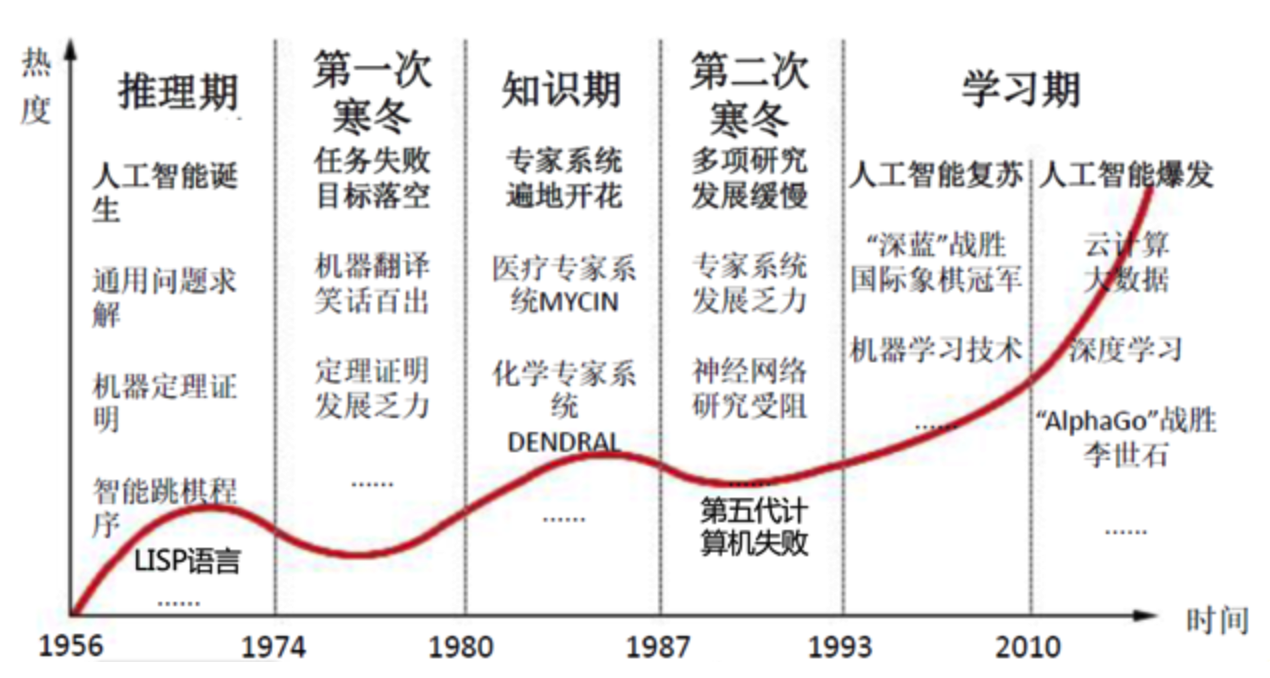
\includegraphics{intro_4.png}
    % \caption[人工智能发展历程]{人工智能发展历程}
	% \labfig{人工智能发展历程}
\end{figure}

人工智能的发展史是科学探索、技术创新与社会需求交织的结果。每一个阶段不仅代表了技术的进步,也反映了在不同历史时期内,人类对于智能本质的理解和追求。从机器定理证明到深度学习,从专家系统到自动驾驶,AI的旅程是对人类智慧的不断挑战和超越,展现了无限的可能性和未来的光明。

今天,人工智能(AI)已经与产业紧密结合,成为推动经济发展和社会进步的关键力量。从智能家居、个性化推荐系统,到自动化生产线、精准医疗,AI的应用遍布我们生活的方方面面,极大地提升了生活质量和工作效率。

AI技术的进步不仅使得设备更加智能,也让服务变得更加贴心和高效。例如,在零售业,通过大数据分析和机器学习,商家能够提供个性化的购物体验,推荐顾客可能感兴趣的商品;在医疗领域,AI能够帮助医生分析病历、诊断疾病,甚至在某些情况下,AI的诊断准确率超过了人类专家。

此外,AI在教育、交通、金融等领域的应用,也正在改变我们的生活方式和工作模式。在线教育平台使用AI来个性化课程内容,适应不同学生的学习速度和风格;智能交通系统能够优化交通流量,减少拥堵;而在金融行业,AI则被用于风险评估、欺诈检测和算法交易等。

尽管AI带来了诸多便利和进步,但它也引发了关于隐私、安全和就业等方面的讨论。随着AI技术的不断发展,如何平衡技术创新与伦理道德的问题,将是我们必须面对的挑战。

\subsection[现状和影响]{现状和影响\sidenote{从国际视角到国内视角,介绍取得的主要成就}}

在过去的六十余年中,人工智能技术经历了显著的演变和进步。特别是在移动互联网、大数据、超级计算、传感网络以及脑科学等领域的新理论和新技术的推动下,人工智能的发展得到了加速。这一时期,由经济和社会发展的强烈需求所驱动,人工智能展现了深度学习、跨界融合、人机协同、群智开放、自主操控等新的发展特征。大数据驱动的知识学习、跨媒体协同处理、人机协同增强智能、群体集成智能、自主智能系统等成为人工智能发展的焦点。受脑科学研究成果的启发,类脑智能正在蓄势待发,而人工智能技术的芯片化、硬件化、平台化趋势更加明显。当前,人工智能的发展已经进入了一个新的阶段,这个阶段特征为新一代人工智能相关学科的发展、理论建模、技术创新以及软硬件的升级等方面的整体推进,引发了链式的突破,并推动了经济社会各领域从数字化、网络化向智能化的加速跃升。

人工智能已成为全球竞争的新焦点。作为引领未来的战略性技术,世界主要发达国家已将人工智能的发展视为提升国家竞争力和维护国家安全的重要战略。这些国家加快出台规划和政策,围绕核心技术、顶尖人才、标准规范等方面强化部署,力图在新一轮的国际科技竞争中掌握主导权。在这一背景下,各国在人工智能领域的投资和研究不断加强,推动了一系列创新和突破,包括自动驾驶汽车、智能家居、智能医疗、机器人技术等领域的快速发展。

面对新形势新需求,为了把握人工智能发展的重大历史机遇,中国的人工智能发展已经被确定为国家战略。中国的最高领导人习近平、李克强对人工智能和机器人学的发展给予了高度的指导和支持。习近平总书记在2014年的讲话中强调了大数据、云计算、移动互联网以及机器人技术的融合发展,以及人工智能领域的迅速进步,这标志着中国对于人工智能及其相关技术的高度评价和对开发这些技术的强烈推动。在这个基础上,中国加大了在人工智能基础研究和应用研究的投资,致力于在人工智能的关键技术和应用领域取得突破,从而在全球人工智能竞争中占据有利地位。

\begin{marginfigure}[-5.5cm]
	
\includegraphics{intro_5.png}
	\caption[中国的人工智能发展已经被确定为国家战略]{中国的人工智能发展已经被确定为国家战略}
\end{marginfigure}

这些年,中国在人工智能领域取得了显著成就,这标志着国家在科技创新和应用实践方面迈出了坚实的步伐。语音和图像识别技术的进步极大地优化了人机交互体验,使得智能助手和面部识别系统更加普及;自然语言处理技术的发展则极大地提高了机器翻译和智能客服的效率和准确性;智能推荐系统的完善为电商、娱乐等行业带来了革命性的变化,使得用户体验更加个性化和高效。

在应用领域,智能制造的推广应用提升了生产效率和质量,降低了制造成本,推动了制造业的转型升级。智能医疗不仅提高了医疗服务的效率和准确性,还通过远程医疗等服务,使得优质医疗资源能够惠及更广泛的人群。智慧城市的构建则在提升城市管理效率、改善居民生活质量等方面发挥了重要作用,通过智能交通系统、环境监测等技术的应用,使城市生活更加便捷、环境更加宜居。

这些技术进步和应用的广泛推广,不仅展现了中国在人工智能领域的强大实力,更在实质上提升了国民的生活质量,并且创造了大量的就业和创业机会。随着人工智能技术的持续发展和深化应用,其在教育、农业、金融等更多领域的潜力将被进一步挖掘,为中国的社会经济发展提供更加广阔的空间和可能性。

这一切的成就,归功于国家对人工智能领域的战略引导和持续投入。通过出台相关政策、增加研发资金支持、构建创新生态系统等措施,中国政府为人工智能技术的研究、开发和应用创造了良好的环境,促进了科技创新与产业发展的紧密结合。这种长远布局和坚定决心,不仅促进了国内人工智能产业的快速成长,也使中国在全球人工智能竞争中占据了有利地位,展现了作为一个崛起中的科技大国的雄心和实力。随着人工智能技术的不断进步和应用的持续深化,预期中国将在推动科技创新和经济社会发展方面实现更多突破,为全球科技进步和人类福祉作出更大贡献。

\subsection[未来和展望]{未来和展望\sidenote{人工智能的未来将何去何从:
- 技术方面,加速大模型的训练和推理
- 应用层面,将人工智能技术和现有产业深度结合,挖掘人工智能技术在更多产业中的应用}}

在过去的许多年,我们见证了人工智能技术的跨越式发展,看到了其在应用层面深度融合现有产业、持续开创新的应用领域的无限可能。随着计算能力的提升、数据量的爆炸式增长以及算法的不断创新,人工智能正在逐步转化为一种基础设施,深刻影响着经济、设计和文化的方方面面。

技术层面上,人工智能的未来将聚焦于加速大模型的训练和推理过程,优化模型效率和可扩展性,同时增强模型的解释性和透明度。通过硬件加速器的创新、新型算法的开发以及云计算和边缘计算的结合使用,未来的人工智能将能够处理更加复杂的任务,实现更高效、更智能的决策和分析。此外,随着人们对于人工智能决策过程的透明度和可解释性要求的提高,提升模型的可解释性将成为重要的研究方向,以确保技术的公平性、安全性和可靠性。

应用层面上,人工智能技术将与各行各业深度结合,推动产业升级和经济结构的优化。在传统行业如制造业、农业、医疗健康等领域,人工智能将通过优化生产流程、提升服务效率和质量、实现个性化需求的满足,来推动这些行业的数字化转型。同时,人工智能也将开辟新的应用领域,如情感计算、虚拟现实、智能交通等,通过这些创新应用,不仅能够改善人们的生活质量,还有助于解决社会、环境等全球性挑战。

随着技术的持续进步和社会的广泛接纳,人工智能的未来充满了无限可能。它不仅会继续推动技术界的革新,更将在更广泛的层面上,促进社会的进步和人类生活方式的转变。面对这样一个充满潜力和挑战的未来,持续的创新、负责任的部署以及跨领域的合作将是推动人工智能健康、可持续发展的关键。

\subsection{问题与反思}
人工智能产业的发展虽然迅猛,但其成长路径上仍面临多项挑战和问题。这些问题不仅关系到技术本身的进步和优化,还涉及伦理、社会和法律等多个维度。以下是一些人工智能产业需要特别关注的问题:
1. 数据隐私和安全:随着人工智能系统对数据的依赖日益增加,如何保护个人隐私和数据安全成为一大挑战。这不仅需要强大的技术解决方案,还需要相应的法律法规和标准来规范数据的收集、使用和分享。
2. 伦理和责任:人工智能的决策过程往往是黑箱的,这引发了关于其决策基础和伦理标准的担忧。如何确保人工智能系统的决策是公正、透明并可解释的,以及在出现错误时如何追究责任,是亟需解决的问题。
3. 技术偏见和公平性:人工智能系统可能会因为训练数据的偏见而产生歧视性的决策,这对于推动社会公平具有潜在的负面影响。确保人工智能系统的公平性和无偏见,要求从数据收集、模型训练到结果评估的全过程进行严格的控制和审核。
4. 就业影响:人工智能技术的发展和应用可能会对劳动市场造成冲击,特别是对于那些重复性高、技能要求低的职业。如何在推进人工智能发展的同时,确保就业机会的公平分配和劳动力的平稳转型,是一个重要议题。
5. 技术壁垒和市场垄断:随着少数大公司在人工智能领域的技术积累和市场控制力增强,存在形成新的技术壁垒和市场垄断的风险。这可能限制创新的空间,增加进入门槛,对整个产业的健康发展构成挑战。
6. 国际合作与竞争:在全球范围内,不同国家和地区在人工智能的发展水平、应用领域和政策制定上存在差异。如何在保护国家安全和促进技术自由交流之间找到平衡,推动国际间的合作而非仅仅是竞争,对于促进全球人工智能产业的健康发展至关重要。

解决这些问题需要政府、产业界、学术界和社会各界的共同努力。通过制定合理的政策和标准、推广伦理指导原则、鼓励开放和透明的技术交流,以及加强国际合作,人工智能产业可以在解决这些挑战的同时,继续保持健康和持续的发展。

\section{结语}

人工智能(AI)技术自1956年提出以来,已经经历了从理论探索到实际应用、从初步发展到技术成熟的演变过程。在技术层面,AI涵盖了符号主义、联结主义和行为主义等多个学派,旨在通过模拟和扩展人类智能,实现机器的自我学习、推理和决策。从弱人工智能到探索强人工智能的旅程中,AI技术已经在语音识别、图像处理、自然语言处理等领域取得了显著进步,且不断向其他领域扩展。

AI的发展受益于计算能力的提升、大数据技术的进步和算法的不断创新,已经成为推动经济、社会和文化深刻变革的关键力量。它不仅优化和改进了现有产业的生产流程和服务模式,而且在医疗健康、智能制造、智慧城市等领域展开了新的应用,极大地提高了效率和生活质量。

然而,AI产业的快速发展也带来了一系列挑战和问题,包括数据隐私和安全、伦理和责任、技术偏见和公平性、就业影响、技术壁垒和市场垄断、国际合作与竞争等方面。这些问题需要通过政府、产业界、学术界和社会各界的共同努力,以及制定合理的政策和标准、推广伦理指导原则、鼓励技术交流和国际合作来共同应对。

展望未来,人工智能将继续在技术和应用层面取得进展,特别是在加速大模型的训练和推理、深化与各行各业的融合等方面。AI的未来不仅在于技术的革新,更在于如何负责任地利用技术,促进社会的公平、安全和可持续发展。随着技术的不断进步和社会认知的深化,人工智能有望为人类带来更加广阔的发展空间和未来可能性。
